\documentclass[a4paper]{article}
\usepackage[T1]{fontenc}			% pacchetto per \chapter
\usepackage[italian]{babel}
\usepackage[italian]{isodate}  		% formato delle date in italiano
\usepackage{graphicx}				% gestione delle immagini
\usepackage{amsfonts}
\usepackage{booktabs}				% tabelle di qualità superiore
\usepackage{amsmath}				% pacchetto matematica
\usepackage{enumitem}				% gestione delle liste
\usepackage{pifont}					% pacchetto con elenchi carini
\usepackage[x11names]{xcolor}		% pacchetto colori RGB
% Link ipertestuali per l'indice
\usepackage{xcolor}
\usepackage[linkcolor=black, citecolor=blue, urlcolor=cyan]{hyperref}
\hypersetup{
	colorlinks=true
}

%\usepackage{showframe}				% visualizzazione bordi
%\usepackage{showkeys}				% visualizzazione etichetta

\begin{document}
	\author{VR443470}
	\title{Basi di dati}
	\date{\printdayoff\today}
	\maketitle
	
	\newpage
	
	% indice
	\tableofcontents
	
	\newpage
		
	\section{Introduzione}
	
	\subsection{Sistemi informativi, informazioni e dati}
	
	Ogni organizzazione è dotata di un \textbf{\emph{sistema informativo}}, che organizza e gestisce le informazioni necessarie per perseguire gli scopi dell'organizzazione stessa. Per indicare la \textbf{porzione automatizzata del sistema informativo} viene di solito utilizzato il termine \textbf{\emph{sistema informatico}}.
	
	Nei sistemi informatici le informazioni vengono rappresentate per mezzo di \emph{dati}, che hanno bisogno di essere interpretati per fornire informazioni. Esiste una differenza sottile tra dato e informazioni. Solitamente i primi, se presi da soli, non hanno significato, ma, una volta interpretati e correlati opportunamente, essi forniscono informazioni, che consentono di arricchire la conoscenza:

	\begin{description}
		\item[\textbf{Informazione}:] notizia, dato o elemento che consente di avere conoscenza più o meno esatta di fatti, situazioni, modi di essere;
		\item[\textbf{Dato}:] ciò che è immediatamente presente alla conoscenza, prima di ogni elaborazione. In informatica, sono elementi di informazione costituiti da simboli che devono essere elaborati.
	\end{description}
	
	\noindent
	\textcolor{Red3}{\textbf{[ESAME] Definizione base di dati}}: Una \textbf{\emph{base di dati}} è una collezione di dati, utilizzati per rappresentare con tecnologia informatica le informazioni di interesse per un sistema informativo.
	
	\newpage
	
	
	
	\subsection{Basi di dati e sistemi di gestione di basi di dati}
	
	Inizialmente, venne adottato un ``\underline{approccio convenzionale}'' alla gestione dei dati. Esso \textbf{sfruttava} la presenza di archivi o \textbf{file per memorizzare} e \textbf{per ricercare dati}. Tuttavia, i metodi di accesso e condivisione erano semplici e banali.\newline
	Infatti, erano presenti numerosi \textbf{problemi}:
	
	\begin{itemize}
		\item[\ding{56}] \textbf{Accesso sequenziale}: la scarsa efficienza nell'accesso ai dati su file rendeva lento l'accesso a tali informazioni;
		\item[\ding{56}] \textbf{Ridondanza}: i dati di interesse per più programmi sono replicati tante volte quanti sono i programmi che li utilizzano, con evidente ridondanza e possibilità di incoerenza;
		\item[\ding{56}] \textbf{Inconsistenza}: una diretta conseguenza della ridondanza. Con la presenza di più copie di un determinato dato, l'eventuale cambiamento di uno solo potrebbe portare a questo effetto;
		\item[\ding{56}] \textbf{Progettazione duplicata}: per ogni programma viene replicata la progettazione.
	\end{itemize}
	
	\noindent
	La \textbf{soluzione} è arrivata negli anni '80 con l'avvento delle \textbf{basi di dati}. Quest'ultime gestiscono in modo integrato e flessibile le informazioni di interesse per diversi soggetti.\newline
	\newline \noindent	
	\textcolor{Red3}{\textbf{[ESAME] Definizione DBMS}}: Un \textbf{\emph{sistema di gestione di basi di dati}} (in inglese \emph{Data Base Management System}, \textbf{DBMS}) è un sistema software in grado di gestire collezioni di dati che siano:
	
	\begin{itemize}
		\item[\ding{52}] \textbf{Grandi};
		\item[\ding{52}] \textbf{Condivise};
		\item[\ding{52}] \textbf{Persistenti}.
	\end{itemize}
	
	\noindent
	\underline{assicurando} allo stesso tempo:
	
	\begin{itemize}
		\item[\ding{72}] \textbf{Affidabilità};
		\item[\ding{72}] \textbf{Privatezza};
		\item[\ding{72}] \textbf{Accesso efficiente}.
	\end{itemize}

	Il \textbf{vantaggio} di utilizzare un DBMS è stato evidenziato nella definizione. Quindi:
	
	\begin{itemize}
		\item[\ding{51}] \textbf{Maggiore astrazione} poiché le sue funzioni \underline{estendono il \emph{file system}}, fornendo la possibilità di accesso condiviso agli stessi dati da parte di più utenti e applicazioni;
		\item[\ding{51}] \textbf{Maggiore efficacia} poiché le operazioni di accesso ai dati si basano su un linguaggio di interrogazione.
	\end{itemize}
	
	
	
	
	\subsection{Linguaggi per basi di dati}
	Su un DBMS è possibile specificare operazioni di vario tipo, ma principalmente si distinguono in due categorie:

	\begin{itemize}
		\item \textbf{Linguaggi di definizione dei dati} (\emph{Data Definition Language}, abbreviato con \textbf{DDL}) utilizzati per \underline{definire} gli \underline{schemi logici}, \underline{esterni} e \underline{fisici} e le \underline{autorizzazioni per l'accesso};
		\item \textbf{Linguaggi di manipolazione dei dati} (\emph{Data Manipulation Language}, abbreviato con \textbf{DML}) \underline{utilizzati} per l'\underline{interrogazione} e l'\underline{aggiornamento} delle \underline{istanze} di basi di dati:
		\begin{itemize}
			\item \emph{Linguaggio di interrogazione}, estrae informazioni da una base di dati (SQL, algebra relazionale);
			\item \emph{Linguaggio di manipolazione}, popola la base di dati, modifica il suo contenuto con aggiunte, cancellazioni e variazioni sui dati (SQL).
		\end{itemize}
	\end{itemize}
	
	\newpage
	
	
	
	
	\subsection{Modelli dei dati}
	\textcolor{Red3}{\textbf{Definizione modello dei dati}}: Un \textbf{\emph{modello dei dati}} è un insieme di concetti utilizzati per organizzare i dati di interesse e descriverne la struttura in modo che essa risulti comprensibile ad un elaboratore.
	
	Ogni modello dei dati fornisce \textbf{meccanismi di strutturazione}, analoghi ai \textbf{\emph{costruttori}} di tipo dei linguaggi di programmazione (es: Java), che permettono di definire nuovi tipi sulla base di tipi predefiniti (elementari) e costruttori di tipo. Quindi, i \emph{costruttori} consentono di:
	
	\begin{itemize}
		\item[\ding{43}] \textbf{\emph{Definire}} le \textbf{strutture dati che conterranno le informazioni} della base di dati;
		\item[\ding{43}] \textbf{\emph{Specificare}} le \textbf{proprietà che dovranno soddisfare le istanze} di informazione che saranno contenuto nelle strutture dati.
	\end{itemize}

	\noindent \newline
	\textcolor{Red3}{\textbf{Definizione schemi e istanze}}: È molto importante distinguere gli \textbf{schemi} e le \textbf{istanze} dal concetto di modello dei dati:
	
	\begin{itemize}
		\item \textbf{\emph{Schema}}: parte \underline{invariante nel tempo}, è costituita dalle caratteristiche dei dati. In altre parole, è la descrizione della struttura e delle proprietà di una specifica base di dati fatta utilizzando i costrutti del modello dei dati;
		\item \textbf{\emph{Istanza} o \emph{stato}}: parte \underline{variabile nel tempo}, è costituita dai valori effettivi. Quest'ultimi, in un certo istante, popolano le strutture dati della base di dati.
	\end{itemize}

	\begin{figure}[!htp]
		\centering
		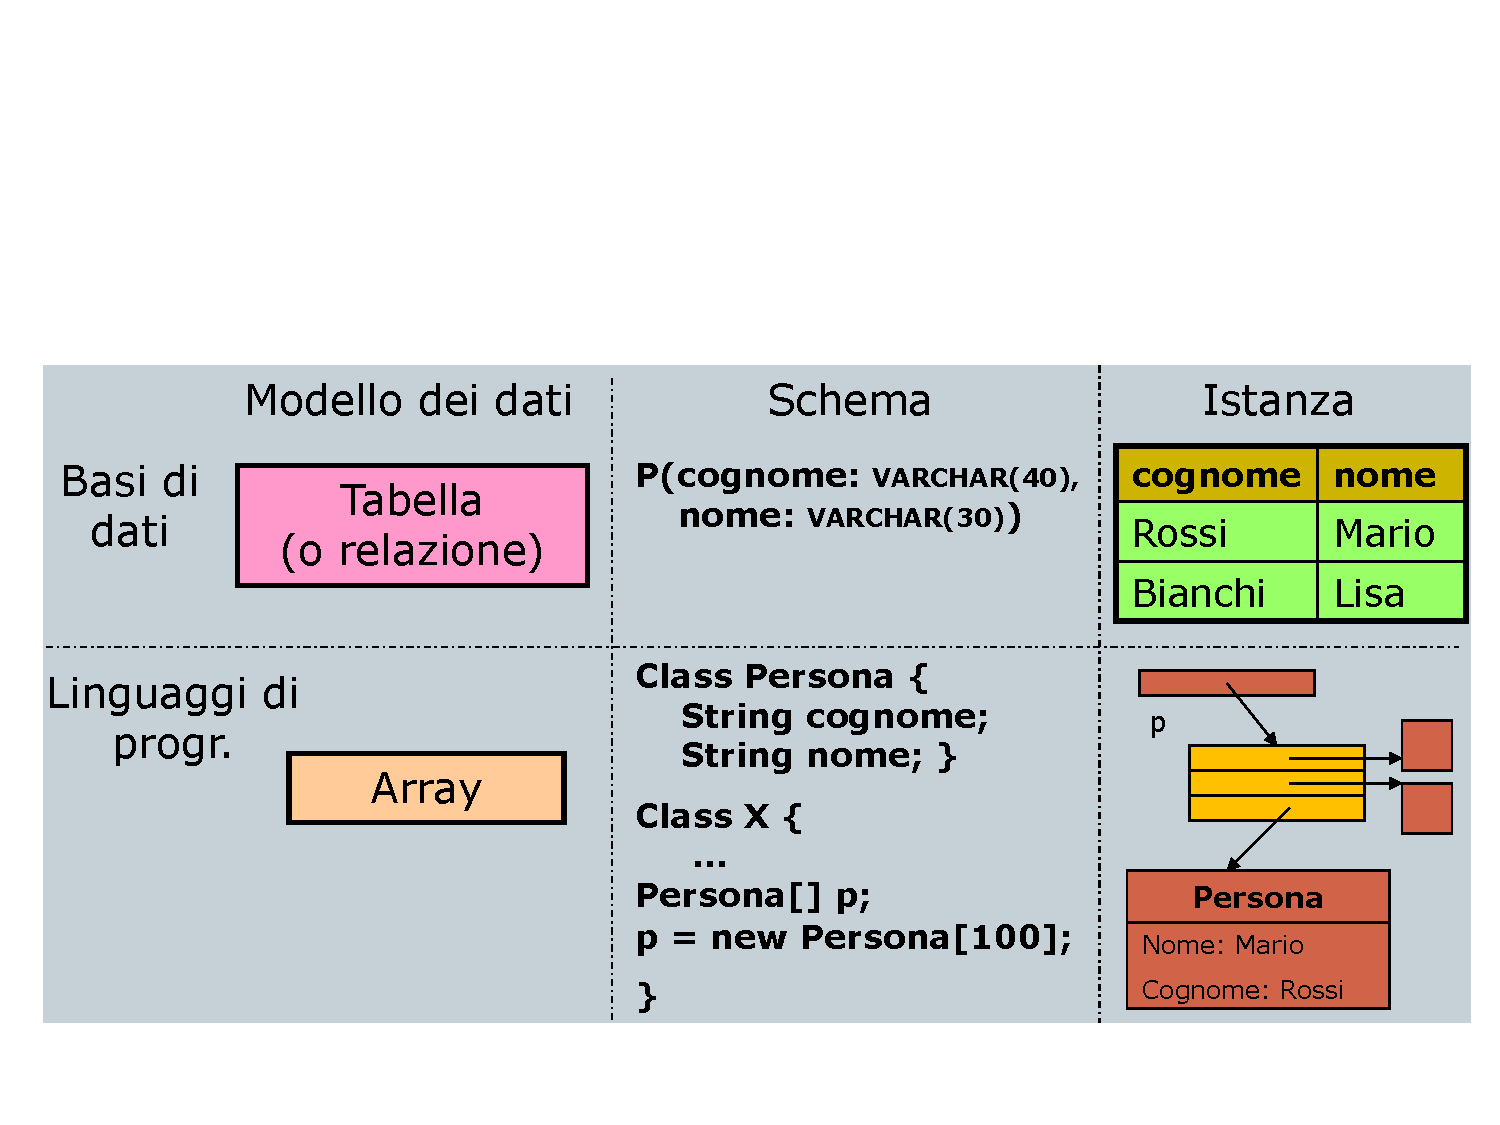
\includegraphics[width=0.9\textwidth]{img/diff_modello-schemi-istanze.pdf}
		\caption{Esempio di modello di dati, schema e istanza.}
	\end{figure}

	\newpage
	
	
	
	
	\subsection{Astrazione (architettura) dei DBMS}\label{Astrazione (architettura) dei DBMS}
	
	Esiste un'architettura standardizzata per i DMBS, la quale si caratterizza su tre livelli: \textbf{esterno}, \textbf{logico} e \textbf{interno}:
	
	\begin{itemize}
		\item[\ding{80}] \textbf{\emph{Schema logico.}} È la rappresentazione della \textbf{struttura} e delle \textbf{proprietà} della \textbf{base di dati} definita \underline{attraverso i costrutti} del modello dei dati del DBMS. In altre parole, descrive l'intera base di dati per mezzo del modello logico adottato dal DBMS (quindi relazione o ad oggetti).
		
		\item[\ding{72}] \textbf{\emph{Schema interno.}} È la rappresentazione della base di dati per mezzo delle \textbf{strutture fisiche di memorizzazione} (e.g. file sequenziale, file hash, ecc.).
		
		\item[\ding{73}] \textbf{\emph{Schema esterno.}}\label{schema esterno} Descrive una \textbf{porzione dello schema logico} di interesse per uno \textbf{specifico} utente o applicazione. \underline{Possono esistere più schemi} esterni che consentono di avere \underline{punti di vista differenti} senza cambiare la logica di base.
	\end{itemize}

	\begin{figure}[!htp]
		\centering
		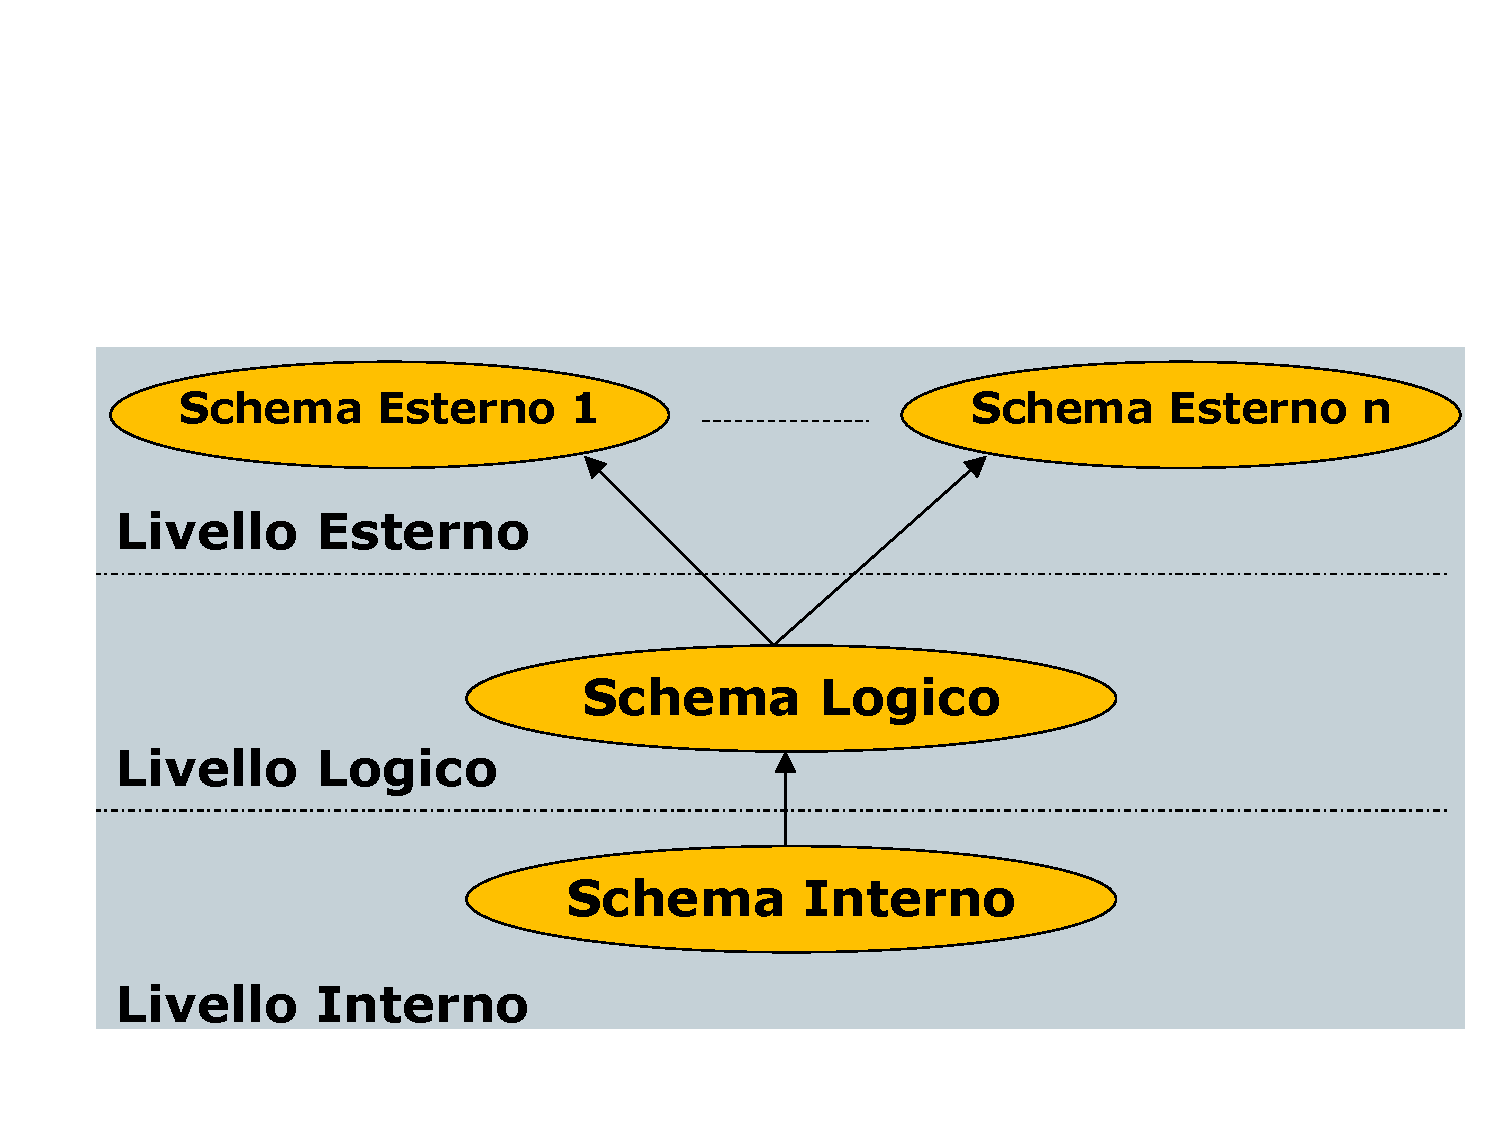
\includegraphics[width=0.8\textwidth]{img/arch_DBMS.pdf}
		\caption{Architettura generale di un DBMS.}
	\end{figure}

	\newpage
	
	
	
	
	\subsection{Indipendenza dei dati}
	
	L'architettura a livelli definita nel paragrafo \ref{Astrazione (architettura) dei DBMS} garantisce l' \textcolor{Red3}{\textbf{indipendenza dei dati}}, la \textbf{proprietà più importante} dei DBMS. L'\textbf{obbiettivo} è quello di poter fornire all'utente una basi di dati in grado di interagire con un \underline{elevato livello di astrazione}. Esistono due tipi di indipendenza:
	
	\begin{itemize}
		\item[\ding{42}] \textbf{\emph{Indipendenza \underline{fisica}.}} Lo schema logico della basi di dati è \underline{completamente} indipendente dallo schema interno. Quindi, l'interazione con il DBMS può essere effettuato in modo indipendente dalla struttura fisica dei dati.\newline
		\textcolor{Green4}{\textbf{Vantaggio:}} le modifiche \textbf{\underline{non}} influiscono sullo schema logico, cioè sulle applicazioni che lo utilizzano.
		
		\item[\ding{42}] \textbf{\emph{Indipendenza \underline{logica}.}} Gli \underline{schemi esterni} (definizione nel paragrafo:~\ref{schema esterno}) della base di dati sono \textbf{\underline{indipendenti}} dallo \underline{schema logico}. Quindi, è possibile interagire con il livello esterno in modo indipendente dal livello logico.\newline
		\textcolor{Green4}{\textbf{Vantaggio:}}
		\begin{enumerate}[label=\Roman*]
			\item \textbf{Aggiunta/Modifica} di uno schema \underline{esterno} in base alle esigenze di un nuovo utente, senza modificare lo schema logico;
			
			\item \textbf{Modifica} di uno schema logico mantenendo inalterate le strutture esterne.
		\end{enumerate}
	\end{itemize}

	\newpage
	
	


	\section{Metodologie e modelli per il progetto}
	
	\subsection{Ciclo di vita dei sistemi informativi}
	
	La progettazione di una base di dati costituisce solo una delle componenti del processo di sviluppo di un sistema informativo complesso e va quindi inquadrata in un contesto più ampio quello del \textbf{ciclo di vita} dei sistemi informativi:
	
	\begin{itemize}
		\item[\ding{42}] \textbf{\emph{Studio di fattibilità.}} Definisce i \underline{costi} delle varie alternative possibili e stabilisce le \underline{priorità di realizzazione} delle varie componenti del sistema.
		
		\item[\ding{42}] \textbf{\emph{Raccolta e analisi dei requisiti.}} Individua le proprietà e le funzionalità che il sistema informativo deve avere producendo una descrizione completa, ma generalmente informale.
		
		\item[\ding{42}] \textbf{\emph{Progettazione.}} Si divide in due fasi:
		\begin{itemize}
			\item \textbf{Progettazione dei dati.} Individua la struttura e l'organizzazione che i dati devono avere.
			
			\item \textbf{Progettazione delle applicazioni.} Definizione delle caratteristiche dei programmi applicativi.
		\end{itemize}
		
		\item[\ding{42}] \textbf{\emph{Implementazione (su un DBMS).}} È la realizzazione del sistema informativo secondo la struttura e le caratteristiche fornite durante la fase di progettazione. In questa fase \underline{viene costruita e popola la base di dati}.
		
		\item[\ding{42}] \textbf{\emph{Validazione e collaudo.}} Verifica il corretto funzionamento e la qualità del sistema informativo.
		
		\item[\ding{42}] \textbf{\emph{Funzionamento.}} Il sistema informativo diventa operativo ed esegue i compiti per i quali è stato progettato.
	\end{itemize}

	\noindent
	Spesso il processo \textbf{non} è strettamente sequenziale. Infatti, come si vede dalla seguente figura, durante l'esecuzione di una delle attività sopraelencate, è necessario rivedere decisioni prese nell'attività precedente.
	
	\begin{figure}[!htp]
		\centering
		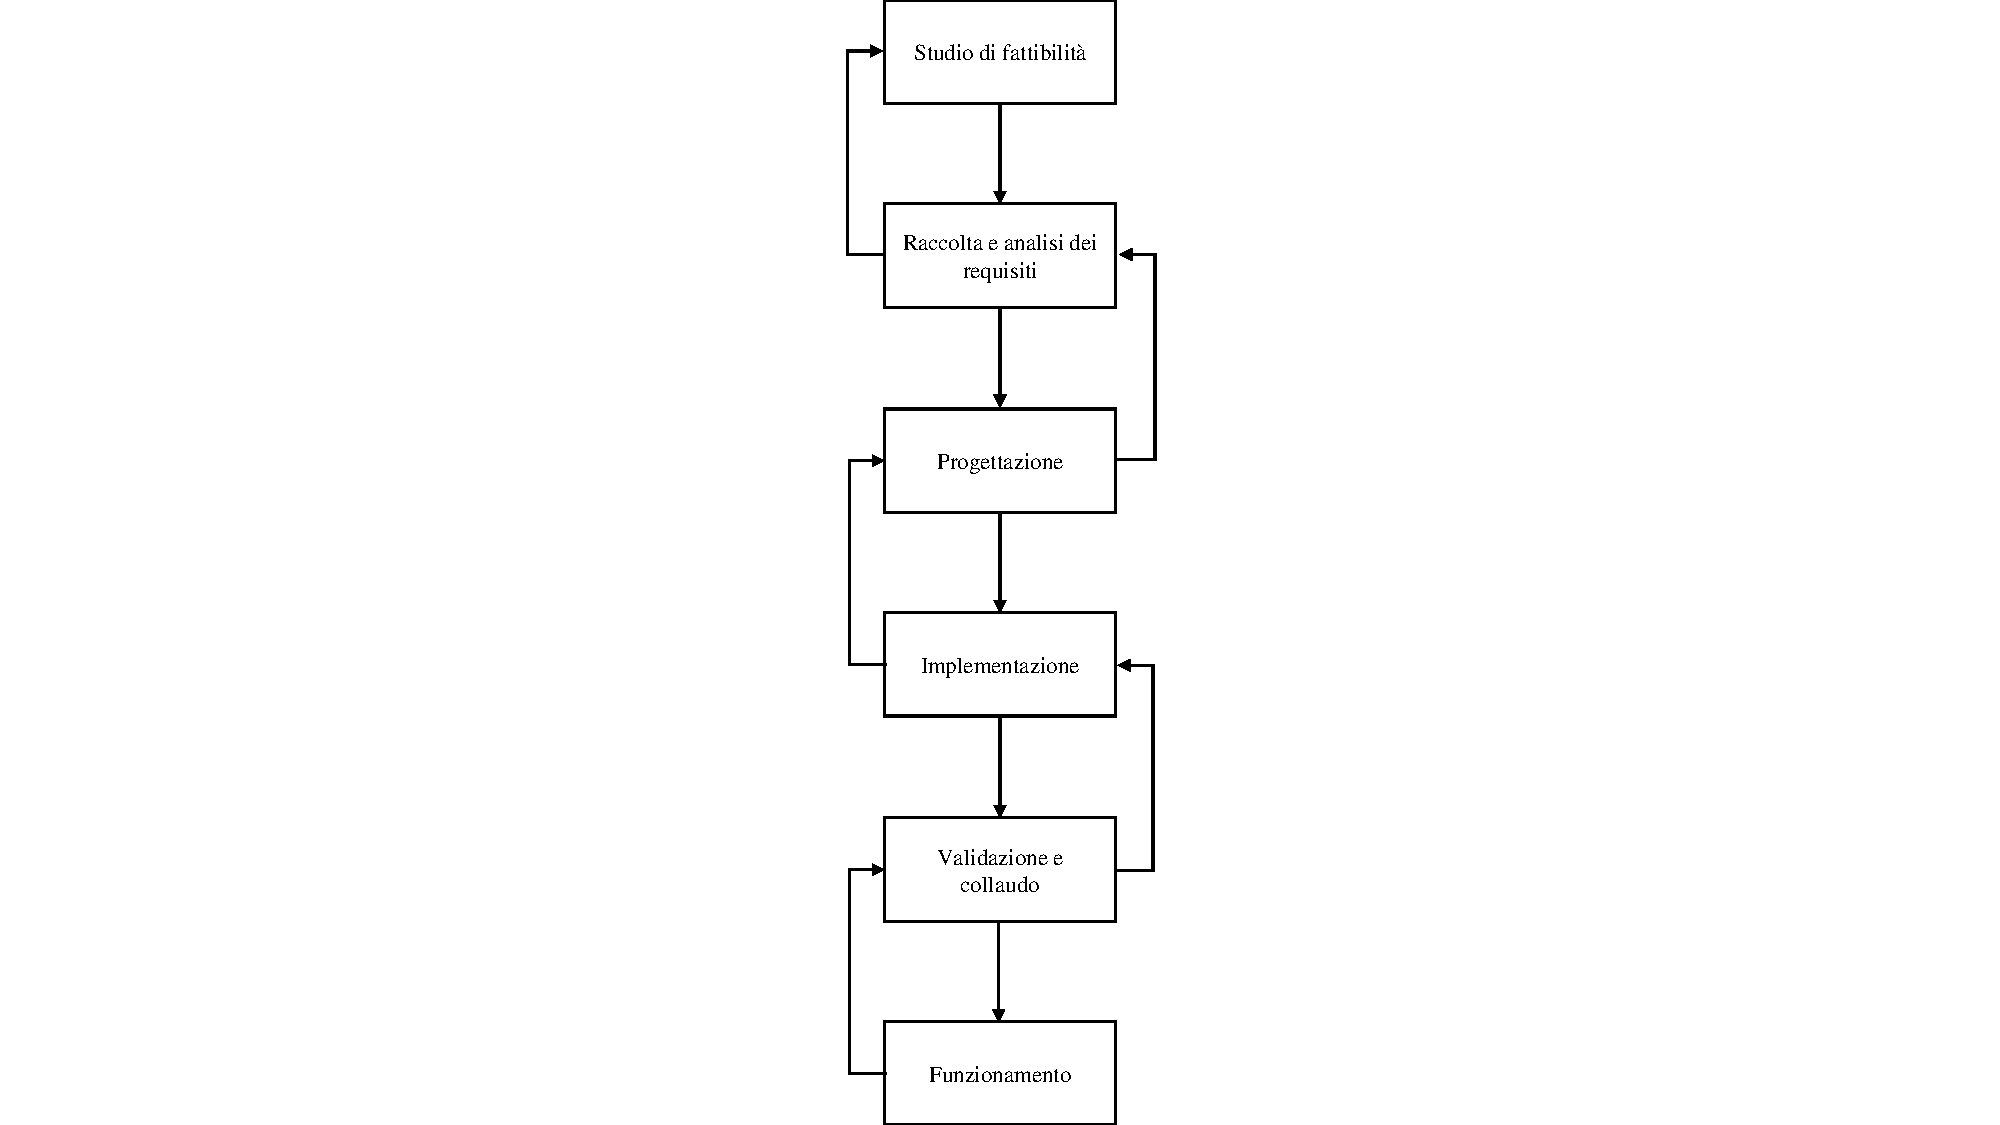
\includegraphics[width=0.4\textwidth]{img/ciclo_di_vita_sis_inf.pdf}
		\caption{Ciclo di vita di un sistema informativo.}
	\end{figure}

	\newpage
	
	
	
	
	\subsection{Metodologie di progettazione e basi di dati}
	
	Una \textbf{metodologia di progettazione} consiste in:
	
	\begin{itemize}
		\item[\ding{51}] \textbf{Decomposizione} dell'intera attività di progetto in passi successivi indipendenti tra loro.
		
		\item[\ding{51}] \textbf{Strategie} da seguire nei vari passi e \textbf{criteri} nel caso di alternative.
		
		\item[\ding{51}] \textbf{Modelli di riferimento} per descrivere i dati in ingresso e uscita delle varie fasi.
	\end{itemize}

	\noindent
	Le \textbf{proprietà} che una metodologia deve garantire sono:
	
	\begin{itemize}
		\item[\ding{72}] \textbf{\emph{Generalità}} rispetto alle applicazioni e ai sistemi in gioco;
		
		\item[\ding{72}] \textbf{\emph{Qualità del prodotto}} in termini di correttezza, completezza ed efficienza rispetto alle risorse impiegate;
		
		\item[\ding{72}] \textbf{\emph{Facilità d'uso}} delle strategie e dei modelli di riferimento.
	\end{itemize}

	%\newpage

	Negli anni si è \emph{consolidata una metodologia} di progetto che ha dato prova di soddisfare pienamente le proprietà descritte. Si basa sull'idea di separare le decisioni relative a ``cosa'' rappresentare in una base di dati (prima fase), da quelle relative a ``come'' farlo (seconda e terza fase):
	
	\begin{itemize}
		\item[\ding{42}] \textbf{Progettazione concettuale.}\newline
		\textcolor{Red3}{\textbf{Obbiettivo:}} rappresentare le specifiche informali della realtà di interesse in termini di una descrizione formale e completa. La \textbf{\underline{rappresentazione}} \textbf{\underline{deve essere indipendente}} dai criteri di rappresentazione utilizzati nei sistemi di gestione di basi di dati.\newline
		\textcolor{Green4}{\textbf{Prodotto di questa fase:}} \underline{schema concettuale}. È un documento formale che rappresenta il contenuto della base di dati in modo indipendente dall'implementazione (DBMS).\newline
		\textcolor{Blue3}{\textbf{Applicazione:}} cercare di rappresentare il \textbf{contenuto informativo} della base di dati, senza preoccuparsi né della modalità con le quali queste informazioni verranno codificate in un sistema reale, né dell'efficienza dei programmi che faranno uso di queste informazioni.
		
		\item[\ding{42}] \textbf{Progettazione logica.}\newline
		\textcolor{Red3}{\textbf{Obbiettivo:}} traduzione dello schema concettuale prodotto nella fase precedente, in termini del modello di rappresentazione dei dati adottato dal sistema di gestione di base di dati a disposizione.\newline
		\textcolor{Green4}{\textbf{Prodotto di questa fase:}} \underline{schema logico}.\newline
		\textcolor{Blue3}{\textbf{Applicazione:}} durante la traduzione, le scelte progettuali si \underline{devono} basare anche su criteri di ottimizzazione delle operazioni da effettuare sui dati.
		
		\item[\ding{42}] \textbf{Progettazione fisica.}\newline
		\textcolor{Red3}{\textbf{Obbiettivo:}} lo schema logico viene completato con la specifica dei parametri fisici di memorizzazione dei dati.\newline
		\textcolor{Green4}{\textbf{Prodotto di questa fase:}} \underline{schema fisico}.\newline
	\end{itemize}
\end{document}